	\paragraph[QuizziPedia::Front-End::ModelViews\\::ProfileManagementModelView]{QuizziPedia::Front-End::ModelViews::ProfileManagementModelView}
	
	\label{QuizziPedia::Front-End::ModelViews::ProfileManagementModelView}
	
	\begin{figure}[ht]
		\centering
		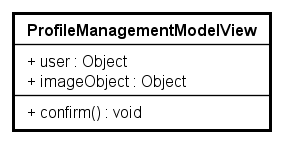
\includegraphics[scale=0.80,keepaspectratio]{UML/Classi/Front-End/QuizziPedia_Front-end_ModelView_ProfileManagementModelView.png}
		\caption{QuizziPedia::Front-End::ModelViews::ProfileManagementModelView}
	\end{figure} \FloatBarrier
	
	\begin{itemize}
		\item \textbf{Descrizione}: classe di tipo modelview la cui istanziazione è contenuta all'interno della variabile di ambiente \texttt{\$scope} di \textit{Angular\ped{G}}. All'interno di essa sono presenti le variabili e i metodi necessari per il \textit{Two-Way Data-Binding\ped{G}} tra la \textit{view\ped{G}} \texttt{ProfileManagementView} e il \textit{controller\ped{G}} \texttt{ProfileManagementController};
		\item \textbf{Utilizzo}: viene utilizzata per effettuare il \textit{Two-Way Data-Binding\ped{G}} tra la \textit{view\ped{G}} \texttt{ProfileManagementView} e il \textit{controller\ped{G}} \texttt{ProfileManagementController} rendendo disponibili variabili e metodi;
		\item \textbf{Relazioni con altre classi}: 
		\begin{itemize}
			\item \textbf{OUT \texttt{ProfileManagementView}}: \textit{view\ped{G}} contenente i dati personali che un utente può modificare dopo essersi registrato al sistema; 
			\item \textbf{OUT \texttt{ProfileManagementController}}: questa classe permette di gestire il profilo personale di un utente.
		\end{itemize}
		\item \textbf{Attributi}: 
		\begin{itemize}
			\item \texttt{+ user: Object} \\ Campo dati contenente i seguenti attributi: \texttt{name: String}, \texttt{surname: String}, \texttt{email: String}, \texttt{image: String}, \texttt{password: String} e \texttt{passwordCheck: String};
			\item \texttt{+ imageObject: Object} \\ Oggetto contenente i seguenti attributi: \texttt{+ imageUrl: String}, \texttt{+ image: Object}.
		\end{itemize}
		\item \textbf{Metodi}: 
		\begin{itemize}
			\item \texttt{+ confirm(user: Object, imageObject: Object): void} \\
			Metodo che gestisce l’evento click sul pulsante di conferma modifica. Aggiorna, in caso di modifiche accettate da sistema, l'oggetto locale \texttt{UserDetailsModel}. Inoltre, utilizzando il metodo dell'\texttt{UserDetailsService}, aggiorna anche nel server i dati dell'utente.
		\end{itemize}
	\end{itemize}	

